\documentclass[review,authoryear,english]{elsarticle}

\usepackage{babel}
\usepackage{natbib}

\bibliographystyle{elsarticle-harv}

\usepackage{lineno}
\usepackage[utf8]{inputenc}  %% Permite utilizar tildes si archivo usa utf-8
\usepackage{amsmath}
\usepackage{amssymb}

\modulolinenumbers[1]

\usepackage{soul}
\usepackage{marginnote}
\usepackage{float}

\usepackage{color}
\definecolor{dkred}{rgb}{0.5,0,0}       %   dark red
\definecolor{todocolor}{rgb}{1.0,0.8,0.5}

\usepackage[hidelinks]{hyperref}

\newcommand{\todohdr}{Please review:}
\newcommand{\TODO}[2][\todohdr]{%
\smallbreak\noindent\colorbox{todocolor}{%
\begin{minipage}{1\linewidth}
\textbf{#1}\par{\footnotesize{#2}}
\end{minipage}}}

\newcommand{\instead}[2]{\textcolor{dkred}{\st{#1}}#2}


%  \usepackage{epstopdf} 
%  \usepackage{epsfig}

\journal{Journal of \LaTeX\ Templates}

\usepackage{subcaption}

\begin{document}

\begin{frontmatter}

\title{Forecasting the black Sigatoka development rate:\\ 
A comparison of machine learning techniques}

%% Group authors per affiliation:
\author[afiLuisAlex]{Luis-Alexander Calvo-Valverde\fnref{myfootnote}}
\ead{lualcava.sa@gmail.com}
\fntext[myfootnote]{Corresponding author. (506)70104420}

\author[afiCorbana]{Mauricio Guzmán-Quesada}
\author[afiCorbana]{José-Antonio~Guzmán-Alvarez}
\author[afiPablo]{Pablo Alvarado-Moya}

\address[afiLuisAlex]{DOCINADE, Instituto Tecnológico de Costa Rica, 
Computer Research Center, Multidisciplinar program eScience, Cartago, Costa Rica}

\address[afiCorbana]{Dirección de Investigaciones, Corporación Bananera Nacional S.A., Guápiles, Costa Rica}

\address[afiPablo]{DOCINADE, Instituto Tecnológico de Costa Rica, Cartago, Costa Rica}

\begin{abstract}
Pending.
\end{abstract}

\begin{keyword}
Machine learning \sep Black Sigatoka \sep Support vector regression \sep
Banana disease prediction \sep Biological warning system 
\end{keyword}

\end{frontmatter}

\linenumbers

\section{Introduction}

The black Sigatoka disease caused by the fungus \emph{Mycosphaerella
  fijiensis Morelet} is the major pathological problem of banana and
plantain crops in Central America, Panama, Colombia and Ecuador, as well as in
many parts of Africa and Asia \citep{MarinVargas1995}.

This disease attacks the plant leaves producing a rapid deterioration
of the leaf area, affects the growth and productivity of the plants
due to the impairment of the photosynthetic process, causes a
reduction in the quality of the fruit, and promotes premature
ripening of bunches, which is
the major cause of product losses associated with the black
Sigatoka. \figurename~\ref{fig:diseasestages} shows three stages of
this disease.
	 
\begin{figure}[ht] 
\centering
\begin{tabular}{c@{\;}c@{\;}c}
  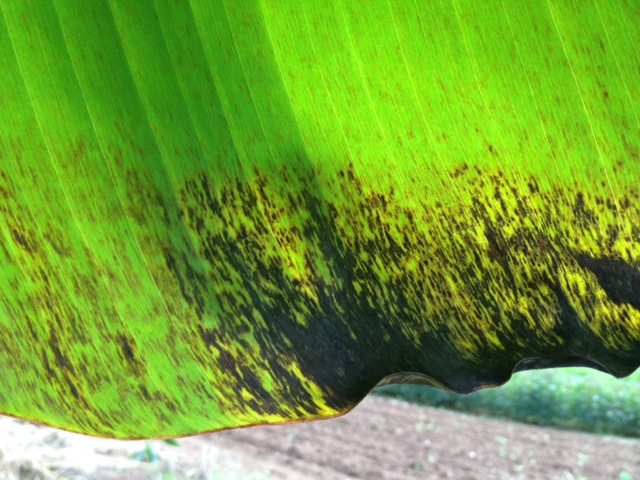
\includegraphics[width=.32\linewidth]{Roya_a} &
  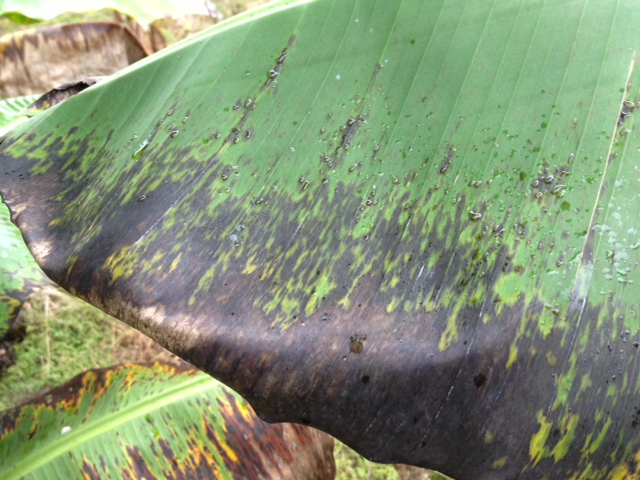
\includegraphics[width=.32\linewidth]{Roya_b} &
  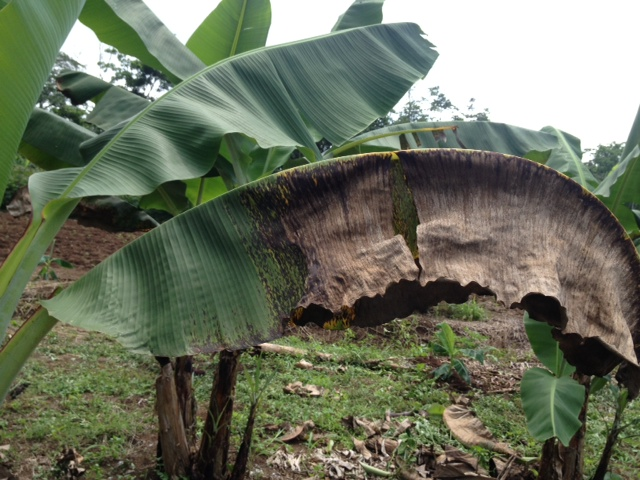
\includegraphics[width=.32\linewidth]{Roya_c} \\
  (a) & (b) & (c) 
\end{tabular}
\caption{Examples of three disease stages of the black Sigatoka. 
(a)~Initial stage. (b)~Intermediate stage, and (c)~Advanced stage.} 
\label{fig:diseasestages} 
\end{figure}

Phytopathological studies point out that precipitation, temperature,
relative humidity and wind are the main climatic variables that affect
the development of this disease \citep{MarinVargas1995}.

In Costa Rica the black Sigatoka is frequently treated with
chemical fungicides.
%
Depending on the zone of production and the weather conditions,
45--55~cycles/year of fungicide applications are required to keep this
disease under control and to produce the expected fruit quality for the
international markets.
%
This represent a cost per hectare per year in the range between US\$1600 and
US\$2000; about 0.64--0.80 cents of the production costs for a
18.14\,kg box.
%
Overall, this represents 10\%--12\% of the total production costs.

The past and present rates of disease development can in principle be used
to predict its future behavior and to determine whether
a particular fungicide spray program will be able to effectively and
economically control the disease \citep{ChuangJeger1987}.

There are efforts to apply machine learning methods to support
decision-making in agriculture, including the control of crop
diseases. For example, \cite{Camargo2012} present an intelligent
system for the assessment of crop disorders, \cite{Huang2010}
introduce a plant virus identification method based on neural networks
with an evolutionary preprocessing stage, \cite{Kim2014} summarize in
their survey crop pests prediction methods using regression and
machine learning approaches, while \cite{Zhao2013} present an
intelligent agricultural forecasting system based on wireless sensor
networks.

In this work, we compare five machine learning techniques 
to predict the development rate of the black Sigatoka disease:
support
vector regression (SVR), echo state networks (ESN), ridge regression,
elastic-net regression and ordinary least squares linear regression.

The main contribution of this work is a comparison between machine
learning methods to forecast black Sigatoka development rate. 
\marginnote{FALTA COMPLETAR esta parte}



\section{Materials and methods}

\subsection{Concepts}

\subsubsection{Black Sigatoka disease}

The black Sigatoka is a disease caused by the fungus
\emph{Mycosphaerella fijiensis Morelet}.  It is the main
phytopathologic problem of banana and plantain crops in Central
America \citep{MarinVargas1995}.
%
This disease attacks the plant leaves producing a rapid deterioration
of the leaf area. It affects the growth and productivity of the
affected plant by impairing its photosynthetic capacity, which
consequently causes a reduction in quality of the fruit
\citep{MarinVargas1995}.

The climate has a major effect on the development of the black
Sigatoka.  Precipitation, temperature, relative humidity and wind are
the main climatic variables affecting the development of this disease
\citep{MarinVargas1995}.

\subsubsection{Biological warning system}


\TODO{Revisar si la nueva redacción de este párrafo coincide con la
  original.  Eso es lo que creo se quería decir, porque no quedaba
  claro cuál sistema fue creado por quién...  Las referencias a cada
  sistema en algo así son absolutamente necesarias.  Favor reemplazar
  \citep{XXX} por las referencias correspondientes (Pablo, 1/5/16)}

The early warning system developed by Ganry and Meyer \citep{XXX} for
the control of the yellow Sigatoka in Cameroon was adapted by Ganry
and Meyer \citep{XXX} for the black Sigatoka. 
%
%The early warning system for black Sigatoka \citep{XXX} is an
%adaptation of the yellow Sigatoka warning system developed by Ganry
%and Meyer \citep{XXX}.  It was modified by Ganry and Laville
%\citep{XXX} for its ito use for controlling yellow Sigatoka in
%Cameroon.
Ternesien and Fouré \citep{XXX} later improved Ganry and Laville's system.

The latter system is based on weekly quantified observations of
the disease progression on young leaves of the plant, according to
Fouré's scale of the symptom stages.
%
The numeric coefficients describe the degree of incidence and the
severity of the disease development.  These coefficients are used to
calculate two variables: gross sum and state of evolution.
\TODO{coefficients??  No suena como coeficientes (un factor que
  multiplica términos en una función) sino como una calificación o
  nota o algo así (quizá ``grade''?).  ``Arbitrary coefficient'' no
  tiene sentido por el ``arbitrary''... No creo que sean tan
  arbitrarios sino predefinidos.  De hecho, el párrafo que sigue dice
  que suben con el avance de síntomas, es decir, no es tan
  ``arbitrario''.  Quizá querés decir ``arbitrarily chosen''?.  No
  estoy seguro si entiendo lo que se quiere decir aquí.}

The gross sum is based on the present disease progression stage and 
\instead{an arbitrary coefficients}{the arbitrarily chosen grading},
which increases with the advance of the symptoms and the
juvenility of the leaf.
%
The state of evolution is calculated using the gross sum and the
foliar emission period.
%
Although threshold levels were initially suggested as a guide to spray
\instead{timing}{schedules}, the fluctuation of these two variables
was found to better define appropiate times to spray
\citep{Marinetal2003}.

\subsubsection{Support Vector Regression (SVR)}

From the perspective of Support Vector Regression (SVR) the regression function $y = f(s)$ for a given dataset $D=\{(s_i,y_i)\}_{i=1}^n$ , is represented as a linear function of the form \citep{Wei2013}:
$$f(s)=w^Ts+b$$
where $w$ and $b$ are respectively the weight vector and the intercept of the model, and they are selected to find an optimal fit to the data available in $D$.

For nonlinear cases, one proceeds by mapping the input p-dimensional vectors via a nonlinear function $\phi : R^p\rightarrow F$, onto the feature space $F$.  After nonlinear mapping, the regression function evolves to a pervasive form:

$$f(s)=w^T \phi (s)+b$$

SVR uses the $\epsilon$-insensitive loss function:
\begin{equation*}
l= {\left| y - f(s) \right| }_{\epsilon } = 
\begin{cases}
   0 & {\left| y - f(s) \right| } \leq \epsilon \\
   \left| y - f(s) \right| - \epsilon & \text{otherwise}
\end{cases}
\end{equation*}
which ignores the error if the difference between the prediction value and the actual value is smaller than $\epsilon$.
%
The $\epsilon$-insensitive loss function allows to find the coefficients $w$ and $b$ by solving a convex optimization problem, which balances the empirical error and the generalization ability.
%
In SVR, the empirical error is measured by the loss function $\epsilon$-insensitive and the generalization ability is measured by the Euclidean norm of $w$ \citep{Cristiani2005}.
%
Then, the optimization problem to identify the regression model can be
formulated by \citep{Wei2013}: 

\begin{equation} 
\begin{aligned}
& \underset{}{\text{minimize}}
& & J(w,\xi_i , \xi_i^* ) = \frac{1}{2}   \Bigr| \Bigr| w \Bigr| \Bigr|^2 + C \sum_{i=1}^{n} (\xi_i , \xi_i^* )    \\
& \text{subject to}
& & \begin{array}{lcl} 
y_i - w^T \phi (s) - b  \leq \epsilon + \xi_i   \\
w^T \phi (s) + b - y_i \leq \epsilon + \xi_i^* & i= 1,2,...,n \\
\xi_i , \xi_i^* \geq 0  \\
\end{array}
\end{aligned}
\end{equation}  
where $C$ denotes the penalty parameter between empirical and generalization errors, and  $\xi_i , \xi_i^*$ are slack variables. \figurename
$.$\ref{figura2} shows this situation.

\begin{figure}[h] 
 \centering
 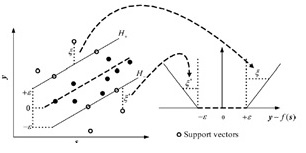
\includegraphics[scale=.9]{SVR}
 \caption{$\epsilon$-insensitive loss function \citep{Wei2013}.} 
 \label{figura2} 
\end{figure}
 
The solution of this optimization problem by the Lagrange method is given by:\\
$$ f(s) = w^T \phi (s) + b = \sum_{i=1}^{n} (\alpha_i - \alpha_i^*) K (s,s_i) + b $$ 
where $\alpha_i - \alpha_i^*$  are the Lagrange multipliers of the optimization problem’s dual form and $K(s_i,s_j )$ is the kernel function satisfying the Mercer condition, and holds:
$$K(s_i,s_j ) = \big \langle  \phi(s_i) , \phi(s_j)  \big \rangle $$
Operations in the kernel function $K(s,s_i )$ are performed in the input space rather than in the potentially high dimensional feature space of $\phi$ \citep{Alonso2013}.

\subsubsection{Ordinary least squares regression}
This method fits a linear model with coefficients $w = (w1,..,wp)$ to minimize the residual sum of squares between the observed responses in the dataset, and the responses predicted by the linear approximation. Mathematically it solves a problem of the form \citep{scikitlearn2011}:
$$\min_{w} \Bigr| \Bigr| Xw - y \Bigr| \Bigr|_2^2  $$
where $X$ denotes the features matriz. \\
According Pedregosa et al. \citep{scikitlearn2011}  the coefficient estimates for Ordinary Least Squares rely on the independence of the model terms. When terms are correlated and the columns of the design matrix $X$ have an approximate linear dependence, the design matrix becomes close to singular and as a result, the least-squares estimate becomes highly sensitive to random errors in the observed response, producing a large variance. This situation of multicollinearity can arise, for example, when data are collected without an experimental design

\subsubsection{Ridge regression}
The ridge regression addresses some of the problems of ordinary least squares regression by imposing a penalty on the size of the coefficients. The ridge coefficients minimize a penalized residual sum of squares  \citep{scikitlearn2011}:

$$\min_{w} { \Bigr| \Bigr| Xw - y \Bigr| \Bigr|_2^2  + \alpha \Bigr| \Bigr| w \Bigr| \Bigr|_2^2 } $$

Here, $\alpha \ \textgreater \  0$ is a complexity parameter that controls the amount of shrinkage: the larger the value of $\alpha$, the greater the amount of shrinkage and thus the coefficients become more robust to collinearity.

\subsubsection{Elastic-Net regression}
Elastic-Net is a linear regression model trained with $L1$ and $L2$ prior as regularizer. This combination allows for learning a sparse model where few of the weights are non-zero like Lasso, while still maintaining the regularization properties of Ridge  \citep{scikitlearn2011}. The convex combination of $L1$ and $L2$ is controled by using the $l1_{ratio}$ parameter.

Elastic-Net is useful when there are multiple features which are correlated with one another. Lasso is likely to pick one of these at random, while elastic-net is likely to pick both.
A practical advantage of trading-off between Lasso and Ridge is it allows Elastic-Net to inherit some of Ridge’s stability under rotation. The objective function to minimize is \citep{scikitlearn2011}:

$$\min_{w} { \frac{1}{2n_{samples}} \Bigr| \Bigr| Xw - y \Bigr| \Bigr|_2^2  + \alpha \rho \Bigr| \Bigr| w \Bigr| \Bigr|_1 + \frac{\alpha (1- \rho)}{2} \Bigr| \Bigr| w \Bigr| \Bigr|_2^2 } $$

\subsubsection{Echo State Networks (ESN)}
Recurrent Neural Networks (RNN) are useful for temporal patterns, but when they are trained with backpropagation methods, they are very slow.  Echo State Network (ESN) is an alternative training method to solve that problem.  ESN is based on the observation that if a random RNN possesses certain algebraic properties, training only a linear readout from it is often sufficient to achieve excellent performance in practical applications \citep{Lukose2009}. 
For a given training input signal $u(n)  \in R^{N_u}$ a desired target output signal $y^{target}(n) \in R^{N_y}$
is known. Here $n = 1, . . . ,T$ is the discrete time and $T$ is the number of data points in the training dataset. The task is to learn a model with output $y(n) \in R^{N_y}$, where $y(n)$ matches $y^target(n)$ as well as possible, minimizing an error measure $E(y,y^target)$, and, more importantly, generalizes well to unseen data. The untrained RNN part of an ESN is called a dynamical reservoir, and the resulting states x(n) are termed echoes of its input history \citep{Lukose2012}. Finally, these signals are sent to an output layer as shown in the \figurename
$.$\ref{figura3}.
\begin{figure}[h] 
 \centering
 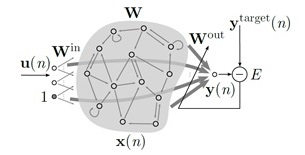
\includegraphics[scale=.9]{Reservorio}
 \caption{An echo state network \citep{Lukose2012}.} 
 \label{figura3} 
\end{figure}
 
The connections between the different elements of an Echo State Network have weights randomly generated. The weights of the internal connections of the reservoir $(W)$ as well as the weights of the input layer $(W_in)$, after being generated are set statically during all stages of implementation of the algorithm. The weights between the reservoir and the output layer $(W_out)$ are subject to changes of a supervised learning algorithm to correct the degree of error generated by the entire system \citep{Lukose2012}.

\subsubsection{Related works}
Huang et al. \citep{Huang2010}  surveyed the development of soft computing techniques in agricultural and biological engineering, including fuzzy logic, artificial neural networks, genetic algorithms, bayesian inference and decision trees.

A related work, proposed by Romero \citep{Romero1995} relies on regression models using a stepwise procedure to predict incubation and latency times of black Sigatoka. The author performed experiments on two farms located in Costa Rica (La Rita and Waldeck, the same as those used in this study but with different names). The study used data from: December 1993 to August 1995. Romero concluded that the model to predict the incubation period accounted a $R^2$ of 69\% in his observed data but it was not a good predictor when it was validated against an independent dataset (cross validation). For latency, he developed two models that accounted a $R^2$ of 78\% in the observed data, however, when validated against an independent dataset (cross validation), for La Rita obtained an adjusted $R^2$ of 82\%, and for Weldeck, none of the models satisfactorily predicted the latent period; and then those predictions were not shown \citep{Romero1995}.

Glezakos et al. \citep{Glezakos2010} proposed to use Genetic Algorithms (GA) and Neural Networks (NN) to identify plant virus (Tobacco Rattle Virus (TRV) and the Cucumber Green Mottle Mosaic Virus (CGMMV)). This is achieved by the development of ana- lytical tools of evolutionary adaptive width, propelled by Genetic Algorithms (GAs) and Neural Networks (NNs). The method was tested against some of the most commonly used classifiers in machine learning (Bayes, Trees and k-NN) via cross-validation and proved its potential towards the identification. 

In the agricultural context, Alves et al. \citep{Alves2011} used  geoinformation techniques to develop predictive models to study the areas of risk to soybean rust in soybean, coffee leaf rust in coffee, and black Sigatoka in banana, considering Brazil’s climatic characterization and the distribution of soybean, coffee and banana crops. Temperature and rainfall data were obtained for the period from 1950 to 2000, and of simulations for 2020, 2050 and 2080 using the SRES A2 climate change scenarios. Using principal components analysis, a single variable was generated based on 57 variables, in order to determine an index explaining 87\%, 88\% and 90\% of the variability of soybean, coffee and banana crops, respectively, in municipal districts across Brazil. The climatic model was used to generate the zoning of the three plant diseases, using temperature and leaf wetness as input. Areas of favorability for the diseases were plotted against the main coffee, soybean and banana growing areas in Brazil. This methodology enabled the visualization of the changes in areas favorable for epidemics under possible future scenarios of climate change.

Other applications of machine learning methods in precision agriculture include the use of support vector regression to predict carcass weight in beef cattle in advance to the slaughter  \citep{Alonso2013}, machine learning assessments of soil drying for agricultural planning \citep{Coopersmith2014}, and early detection and classification of plant diseases with support vector machines based on hyperspectral reflectance \citep{Rumpf2010}.

Furthermore, there have been attempts to generate software tools. Camargo et al. \citep{Camargo2012} presented an information system for the assessment of plant disorders (Isacrodi). They proposed that experts will attain a much better accuracy than the Isacrodi classifier, particularly when provided with samples from the affected crop. However, those cases where such expertise is not available, they suggest that Isacrodi can provide valuable support to farmers. Isacordi includes 15 crop disorders, but the black Sigatoka no is one of them. The prediction process is based on multi-class support vector machines.

Regarding the prediction of the develpment of the black Sigatoka with machine learning methods, Bendini et al. \citep{Bendini2013}  presented a study about the risk analysis of black Sigatoka occurrence based on polynomial models. A case study was developed in a commercial banana plantation located in Jacupiranga, Brazil. It was monitored weekly during the period from February to December 2005. Data included the weekly monitoring of the disease’s evolution stage, time series of meteorological data and remote sensing data. They obtained a model to estimate the evolution of the disease from satellite imagery. This model relates gray levels (NC) of the band 2 images of the Landsat-5 satellite, with the progress status or disease severity (EE). The authors claim to reach an $R^2$ of 90\%.

Also there are works related to banana fruit. Soares et al. \citep{Soares2014} apply two techniques: artificial neural networks (ANNs) and multiple linear regression (MLR) in banana plant to predict the yield, their results show that the neural network proved to be more accurate in forecasting the weight of the bunch in comparison to the multiple linear regressions in terms of the mean prediction-error $(MPE = 1.40)$, mean square deviation $(MSD = 2.29)$ and coefficient of determination $(R^2 = 91\%)$.

In general, the machine learning methods applied to predict the evolution of plant diseases, can be classified in two main approaches: 1) Those whose main inputs are images, and 2) Those whose main inputs are environmental and biological variables. Our study focuses in the second case.

\subsubsection{Data}
In this work we use data acquired in two research farms of Corbana in Costa Rica: 1) 28 Millas (previously called Waldeck and located at Matina) and La Rita (located at Pococí), both in the province of Limón, Costa Rica. The banana type is Musa AAA, subgroup Cavendish, cv. Grande Naine. The \tablename $.$\ref{tabla1} shows the variables available.

\begin{table}[h] 
\caption{Variables used in the study} 
\label{tabla1} 
\centering
\begin{tabular}{c|c} 
\hline
\bfseries Variable & \bfseries Meaning0'0' \\ 
\hline\hline 
$T_{a_{max}}$ &	Max air temperature \\
$T_{a_{min}}$ &	Min air temperature \\
$\overline{T}_{a}$	 & Mean air temperature \\
$\overline{H}$	&  Mean Humidity \\
$H_{min}$ &	Min humidity \\
$H_{max}$	& Max humidity \\
$\overline{R}$	& Mean Solar radiation \\
$P$	& Sum precipitation  \\
$W_{max}$	& Max speed wind \\
$\overline{W}$	& Mean speed wind  \\
$L_2$	& Biological warning system – Leaf 2 \\
$L_3$	& Biological warning system – Leaf 3 \\
$L_4$	& Biological warning system – Leaf 4 \\
$E_s$	& Biological warning system – Evolution Stage \\
\hline
\end{tabular} 
\end{table}

The value to be predicted in all cases was $E_s$, that is the total measure of the biological warning system.  

The data on the biological warning system are collected once a week. Although Corbana has meteorological stations that take data every five minutes, for these experiments, weekly averages generated by nearby stations to each of the farms were used.

The time intervals used for this study were: La Rita, week 48 of 2002 to week 17 of the 2015 (647 weeks) and for 28 Miles, week 37 of 2003 to week 18 of 2015 (605 weeks).

\subsubsection{Data preprocessing}

In 28 Miles farm, 1\% of the data were missing, while in La Rita was 2.25\%. To fill-in the missing values we use spline interpolation. The data collected did not exhibit outliers.

Due the fact that the variables measure meteorological or biological process, they are discretized in order to reflect trends in the data, i.e. the continuous values are not directly used. The coefficient of variation $C_v(x)$ of each variable x was used to determine the number $n$ of discretization levels.
$$n= \lfloor 100 \ C_v(x) \rfloor$$
where $\lfloor \ \rfloor$  is the round operator.

Each discretization range was uniformly partitioned. Besides enabling the capture of tendencies, the discretization removes the effect of small variations in the data collection, either by inaccuracies of the instruments (meteorological variables) or by subjective bias introduced by the human who collects the data (biological warning system). 

Each feature was scaled to fit in a range between 0 and 1. The variable to be predicted was not scaled.

\subsection{Evaluation criteria}

Although there are many types of indicators to assess the quality of the prediction, we selected the determination coefficient $(R^2)$ and the Root Mean Square Error $(RMSE)$.  

Given $n$ records, let be $y$ the actual value of the series, $\hat{y}$ the predicted value and $\acute{y}$ the mean of the observed data.

$$ \bar{y} = \frac{1}{n} \sum_{i=1}^{n} y_i $$

$$ S_e^2 = \frac{\sum_{i=1}^{n} {(y_i-\hat{y}_i)}^2 }{n}$$

$$ S_R^2 = \frac{\sum_{i=1}^{n} {(\hat{y}_i-\bar{y}_i)}^2 }{n}$$

$$ S_y^2 = S_R^2 + S_e^2$$

$$ R^2 = \frac{S_R^2}{S_y^2}$$

$$ RMSE = \sqrt{\frac{\sum_{i=1}^{n} {(y_i-\hat{y}_i)}^2 }{n}}$$
	
This decision is supported by the widespread use in machine learning and agriculture areas \citep{Soares2014}, \citep{Soares2013}, \citep{Ibrahim2014} and \citep{Demir2014}.  

\subsection{Methodology}
The selection of methods and their parametrisation was performed in two stages.

{\bf Phase one } 

In the phase one, we did ten-fold-cross-validation on a set of  machine learning methods and different configurations:

\begin{itemize}
\item 	Patterns: n by m, where n from 1 to 8 and m from 1 to 2.

\item Methods: support vector regression with the kernels functions: linear, gaussian and sigmoid; echo state networks; ordinary least squares linear regression, ridge regression and elastic-net regression.

\item Variables included in the model:
\begin{itemize}
\item All variables.
\item From the set $\{ \overline{T}_{a} , \overline{H}, P , \overline{W}  \}$ use the subsets with one, two or four elements. These variables are according to experts the ones having most impact on the disease development \citep{MarinVargas1995}.
\end{itemize}

\end{itemize}

{\bf Phase two }	

In the second phase, the best configurations obtained in phase one are used to validate with the last 50 and 100 weeks. 

This second phase intents to expose how these methods behave on a considerable climate in the years 2014 and 2015.
\marginnote{Poner una cita que fundamente este ultimo parrafo}

\subsection{Programming environment}

We use the python programming language with the Integrated Development Environment (IDE) Spyder \citep{Continuum2015}, particularly with the libraries pandas \citep{mckinneypandas2010} and numpy \citep{vanderWalt2011}. For SVR, ridge and ordinary least squares regressions, we used sklearn \citep{scikitlearn2011} and for ESN the python-based code of Dr. $Luko\breve{s} evi \breve{c} ius$ \citep{Lukose2012} on which the necessary were done for adjustments for the experiments of this work. The computer used a processor Intel(R) Core i7-4800MQ CPU 2.70GHz, 16.0 GB RAM, running Windows 8 Pro.

\section{Results and discussion}

In this section we present the main results for phase.

{\bf Phase one } 

\figurename $.$\ref{figura4} shows the best $R^2$ for each algorithm in the experiment. Results are group by farm. Though La Rita obtains different results in magnitude than 28 Millas, the trend is similar. In both farms, the best results are for linear models, second position is occupied for Echo State Networks and  SVR with gausian and sigmoid kernels are the worst results. In linear models, to predict one week ahead is better than two weeks ahead, and this is better than three weeks ahead. 

\begin{figure}[H] 
 \centering
 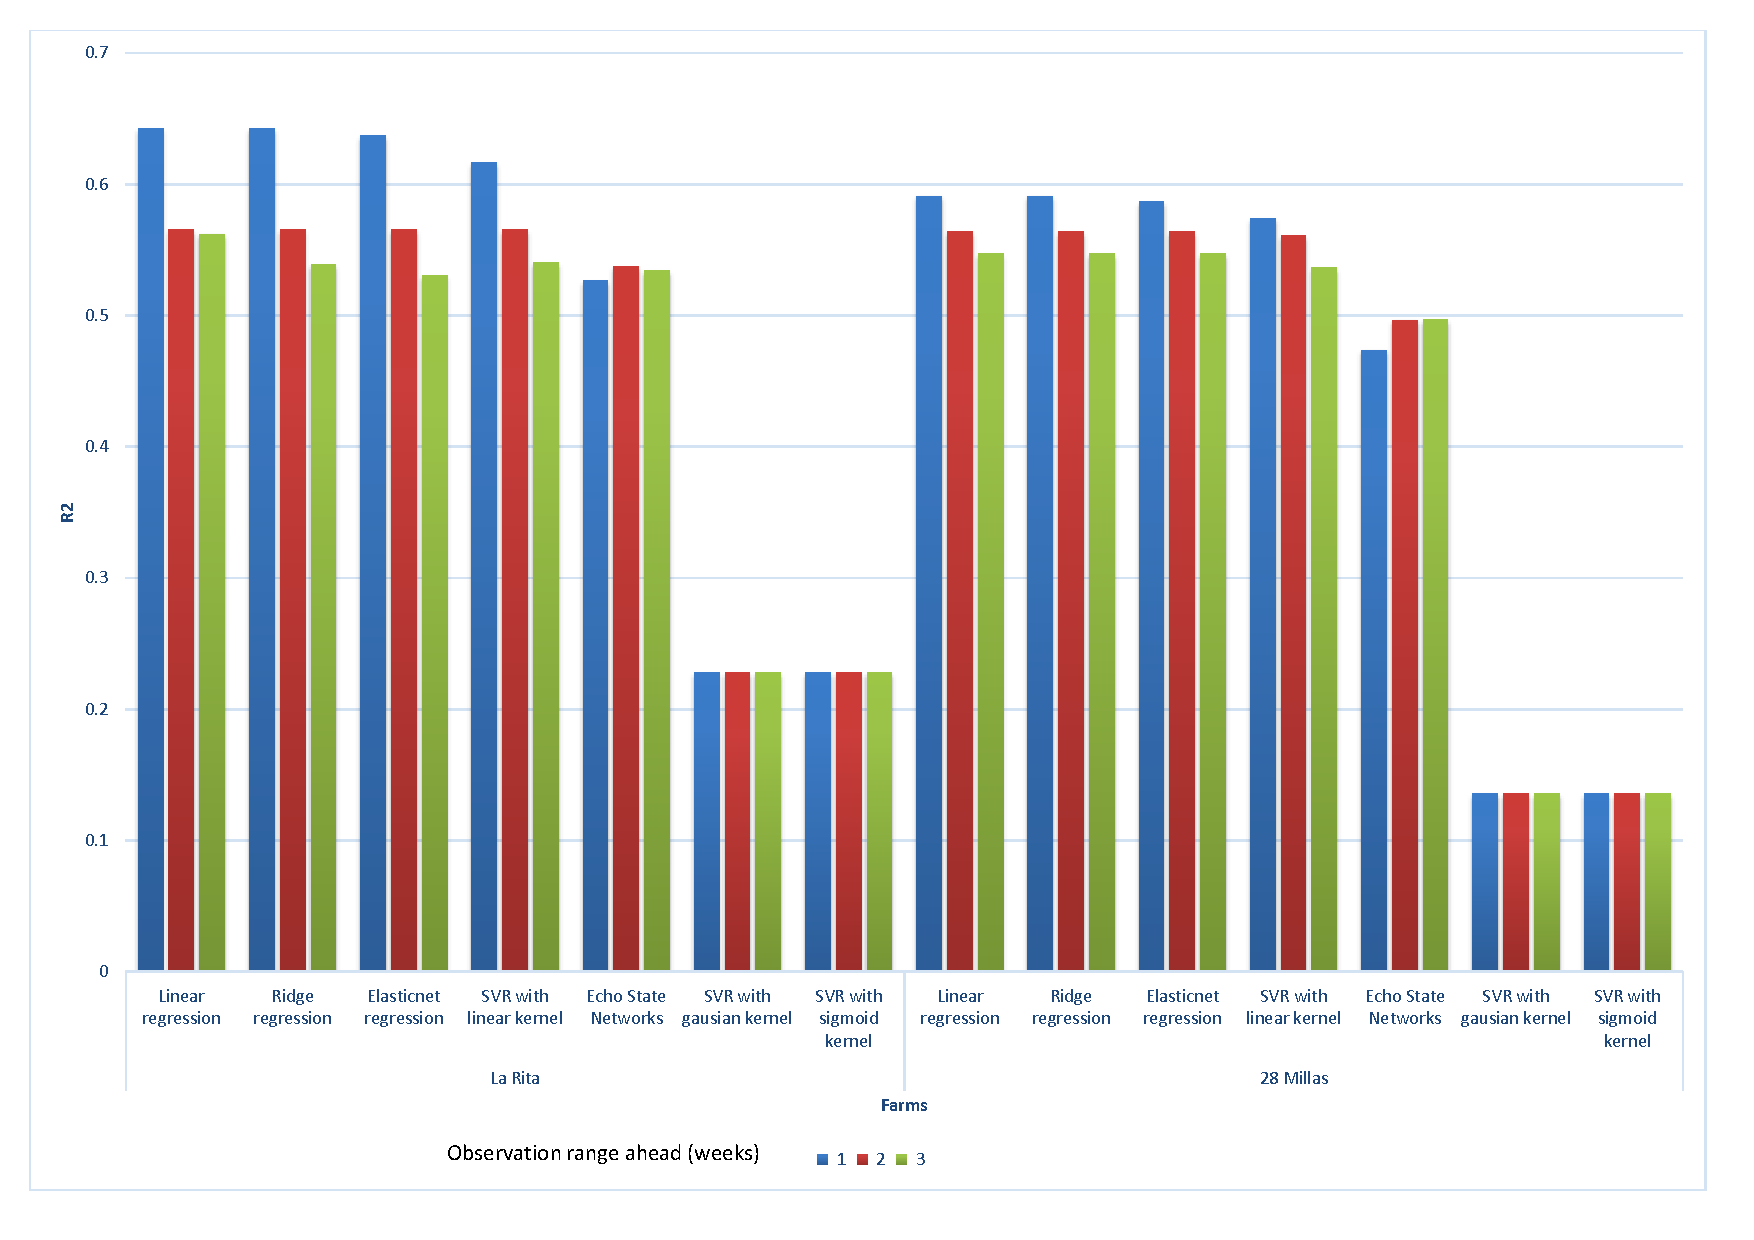
\includegraphics[scale=.5]{Phase_one_Best_R2_for_each_algortihm}
 \caption{Phase one - Best $R^2$ for each algorithm} 
 \label{figura4} 
\end{figure}

\figurename $.$\ref{figura5} presents, for one, two and three weeks ahead, the best $R^2$. Results are group by farm. In general, to predict one week ahead is better than two weeks ahead and so on. The number of weeks consider in the observation range in the pattern is not the main discriminant factor, but it is clear that we get better $R^2$ for one week ahead than two weeks ahead and so on.

\begin{figure}[H] 
 \centering
 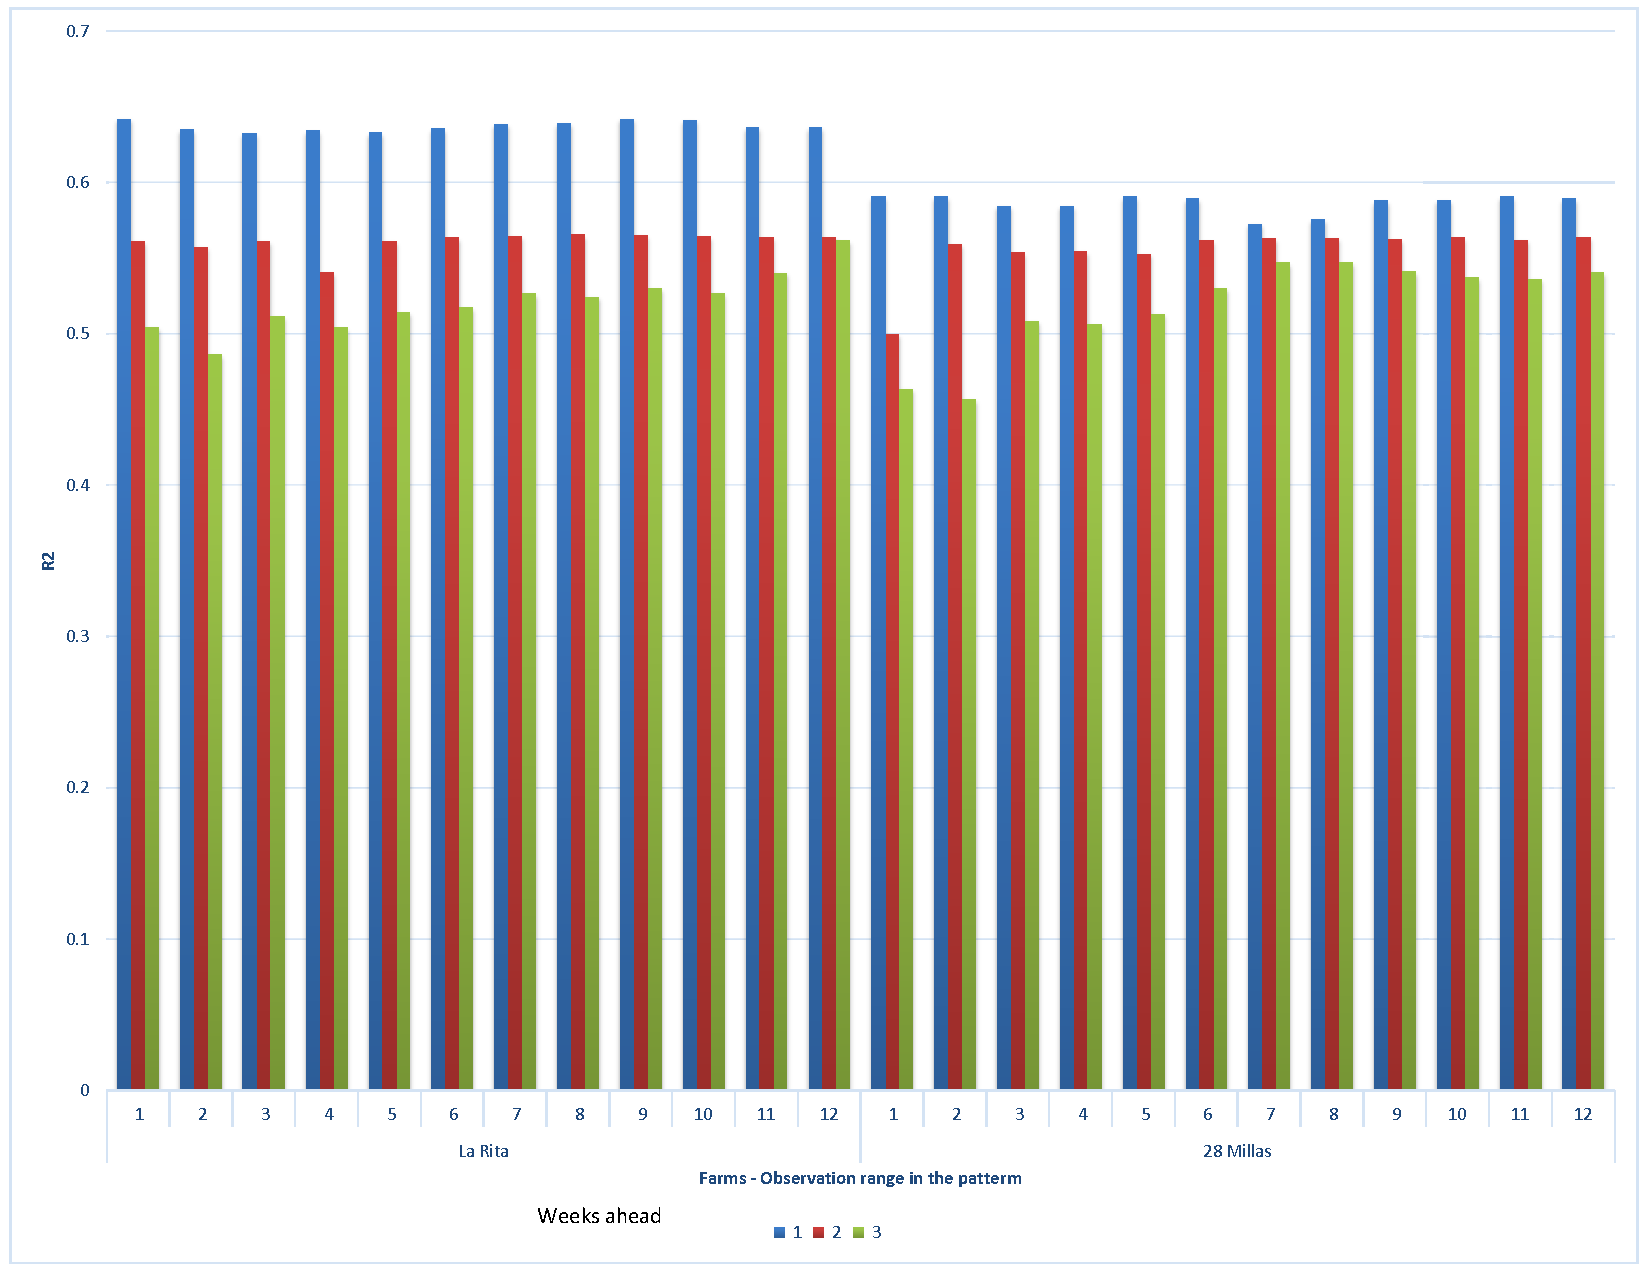
\includegraphics[scale=.5]{Phase_one_Best_R2_for_each_number_of_observation_range_in_the_patterm}
 \caption{Phase one - Best $R^2$ for each observation range} 
 \label{figura5} 
\end{figure}

\figurename $.$\ref{figura6} shows the best $R^2$ for each variables combination. Results are group by farm. The better results are obtained with $\overline{T}_{a}$ and the combination of $\overline{T}_{a}$ with $\overline{W}$, in both farms of similarly. You can note that the use of all variables in the model or the inclusion of the four variables suggest for expert criteria do not improve significantly the results, then the use of more sensors do not assure a better result. 

\begin{figure}[H] 
 \centering
 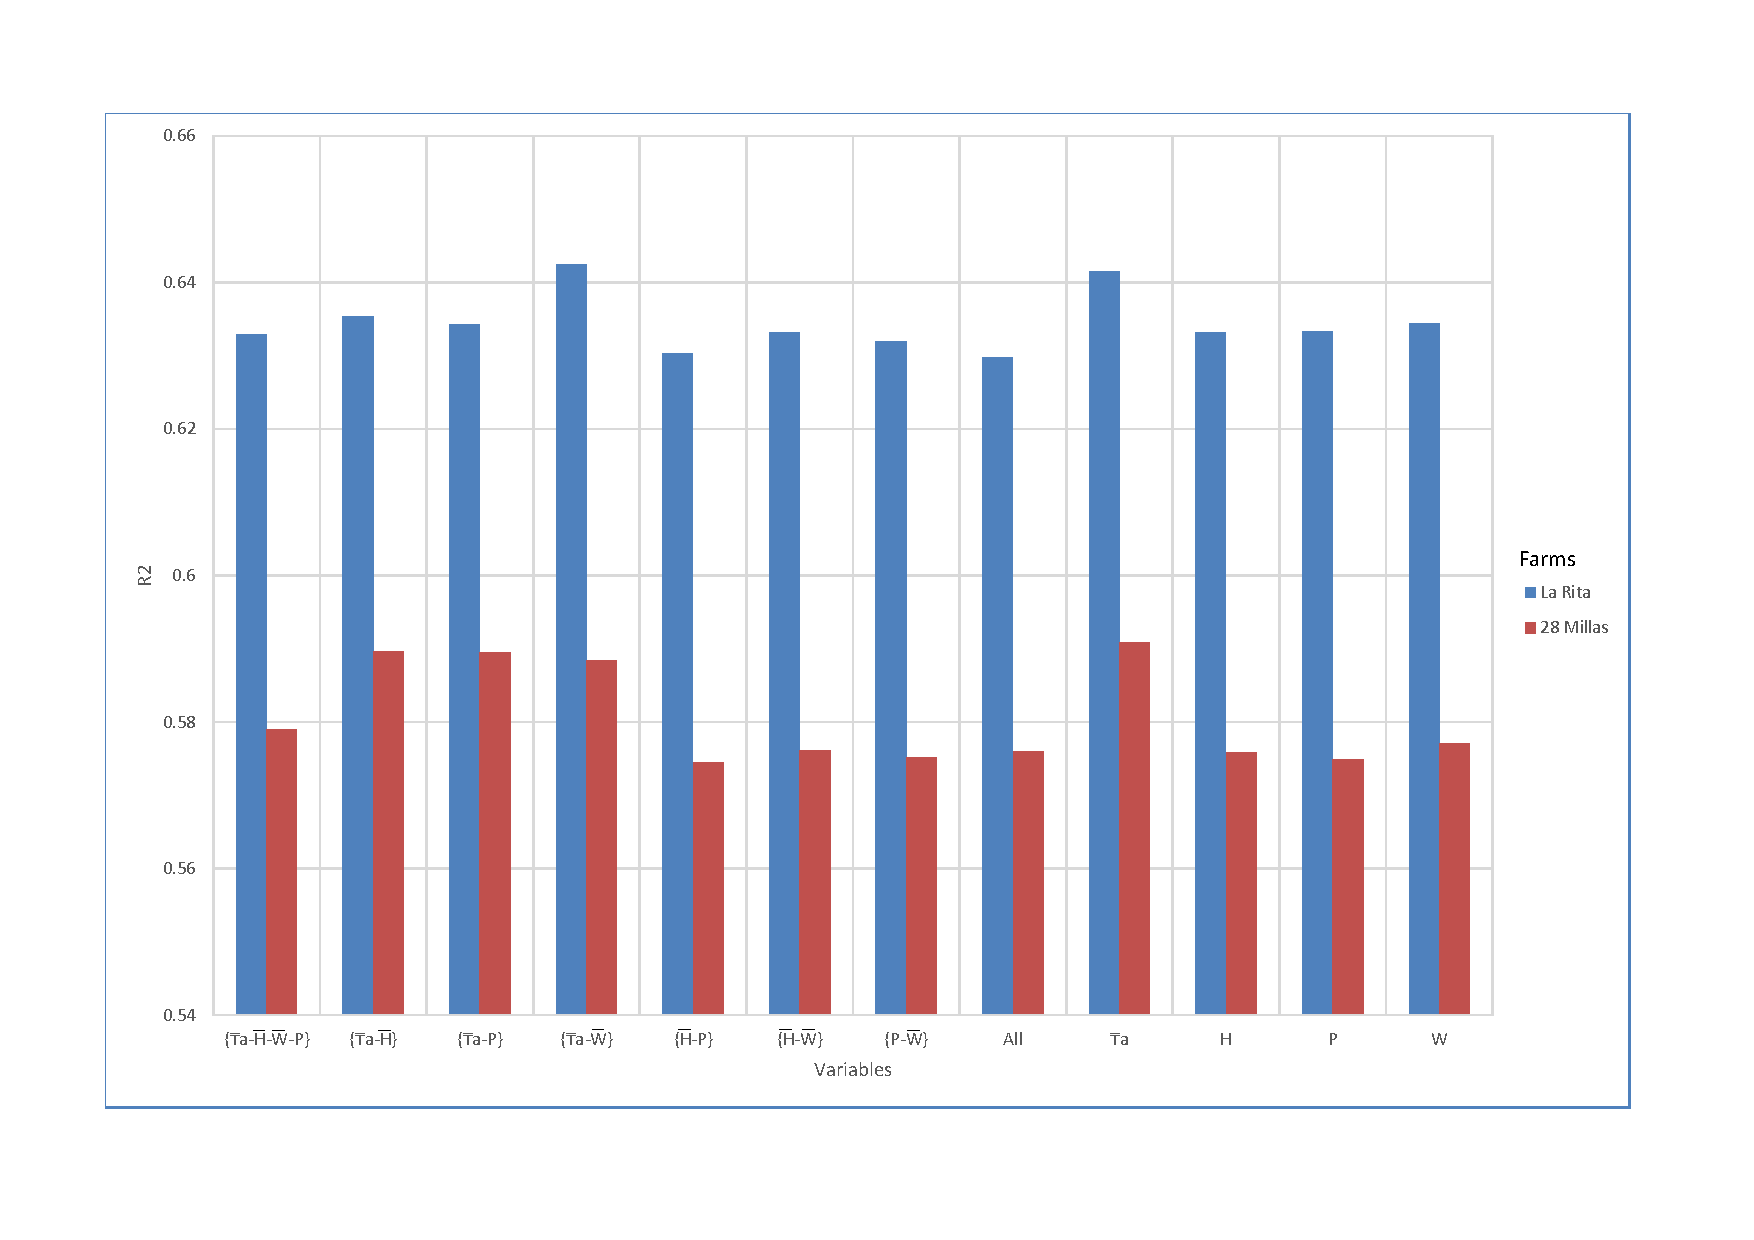
\includegraphics[scale=.5]{Phase_one_Best_R2_for_variables}
 \caption{Phase one - Best $R^2$ for each variable combination} 
 \label{figura6} 
\end{figure}

\figurename $.$\ref{figura7} shows the Pareto frontier for each farm with respect to $R^2$ and $RMSE$. The Rita obtains upper $R^2$ with respect to 28 Millas, but 28 Millas obtains better $RMSE$ than La Rita. This situation arise because $RMSE$ considers errors only with respect the prediction and in 28 Millas the average of Stage of Evolution is $4316.16$, unlike, in La Rita the average is $5507.30$. So, in La Rita we obtains higher errors in absolute values. $R2$ is a relative metric between 0 thru 1 and it is less sensitive to absolute values.

\begin{figure}[H] 
 \centering
 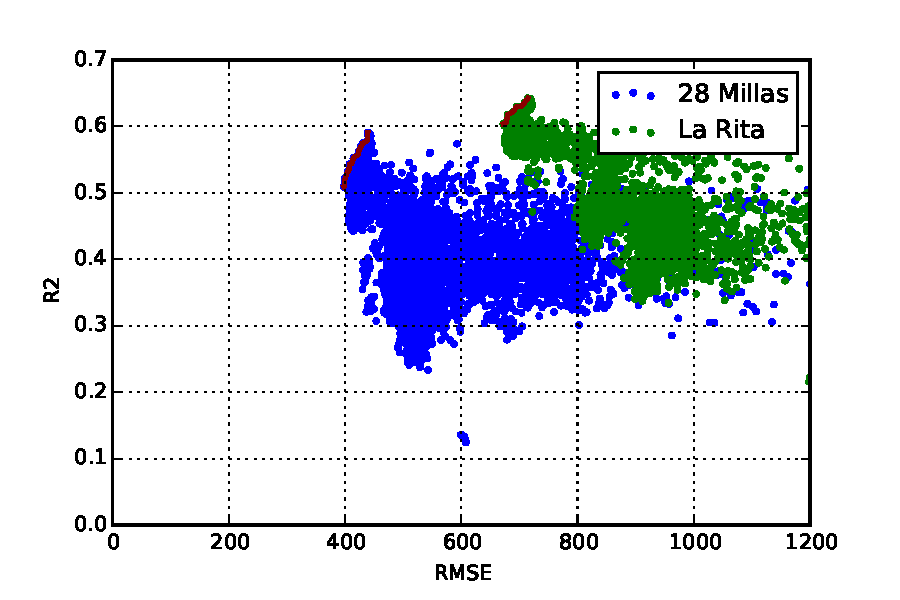
\includegraphics[scale=.8]{Phase_one_R2_RMSE}
 \caption{Phase one - Pareto frontier for $R^2$ and $RMSE$} 
 \label{figura7} 
\end{figure}

The Pareto frontier for the La Rita farm is composed by 96 elements. The \tablename $.$\ref{tabla2} shows the composition about variables and observation ranges.

\begin{table}[h] 
\caption{Composition of the Pareto frontier - La Rita - Phase one} 
\label{tabla2} 
\centering
\begin{tabular}{c|c|c|c|c} 
\hline
\bfseries Variable & \bfseries Observation range & \bfseries Quantity & \bfseries Max $R^2$ & \bfseries Min $RMSE$\\ 
\hline\hline 
Pair $\overline{T}_{a}$ $\overline{W}$ &	1 to 1  & 36 & 64.25\% & 714.51 \\
 &	2 to 1  & 6 & 62.97\% & 695.10 \\
\hline 
All  & 1 to 1  & 18 & 62.98\% & 701.95 \\
   & 2 to 1  & 12 & 61.76\% & 679.92 \\
    & 3 to 1  & 6 & 60.60\% & 676.42 \\
    & 5 to 1  &  2 & 60.37\% & 672.39 \\
\hline    
$\overline{T}_{a}$ & 1 to 1  & 12  & 63.60\% & 708.77 \\
       &	2 to 1  & 4 & 62.23\% & 689.55 \\
\hline
\end{tabular} 
\end{table}

Similarly, the Pareto frontier for the 28 Millas farm is composed by 75 elements. The \tablename $.$\ref{tabla3} shows the composition about variables and observation ranges.

\begin{table}[h] 
\caption{Composition of the Pareto frontier - 28 Millas - Phase one} 
\label{tabla3} 
\centering
\begin{tabular}{c|c|c|c|c} 
\hline
\bfseries Variable & \bfseries Observation range & \bfseries Quantity & \bfseries Max $R^2$ & \bfseries Min $RMSE$\\ 
\hline\hline 
Pair $\overline{T}_{a}$ $\overline{W}$ & 1 to 1 & 8 & 57.80\% & 438.09 \\
\hline 
All   &	9 to 1 & 2 & 50.93\% & 397.93 \\
  & 10 to 1	 & 2 & 50.97\% & 398.81 \\
  &	8 to 1 & 6 & 51.62\% & 398.93 \\
  &	7 to 1 & 2 & 52.25\% & 400.28 \\
  &	6 to 1 & 2 & 53.16\% & 404.14 \\
  &	4 to 1 & 2 & 54.32\% & 407.54 \\
\hline    
$\overline{T}_{a}$ & 1 to 1  & 8  & 59.09\% & 439.44 \\
\hline
Pair $\overline{T}_{a}$ $\overline{H}$ & 1 to 1	 & 8 & 57.51\% & 428.61 \\
 &	2 to 1 & 20 & 56.91\% & 414.37 \\
 &	3 to 1 & 3 & 54.41\% & 411.55 \\
 &	4 to 1 & 3 & 53.34\% & 406.65 \\
\hline
Pair $\overline{T}_{a}$ $P$ & 3 to 1 & 9 & 56.23\% & 422.76 \\
\hline
\end{tabular} 
\end{table}

We can conclude that the best configuration in both farms is to consider the climate and the evolution stage of the current week to predict the evolution stage of the next week.


{\bf Phase two }

In the second phase, the best configurations obtained in phase one were used to validate with the last 50 and 100 weeks. 


\figurename $.$\ref{figura8} shows the best $R^2$ for each algorithm in the experiment. Results are group by farm. Even if linear models continue with good $R^2$, Echo State Networks improve their scores because in $50$ and $100$ last weeks validation, we are in presence of climate change, then the behaviour is less lineal.

\begin{figure}[H] 
 \centering
 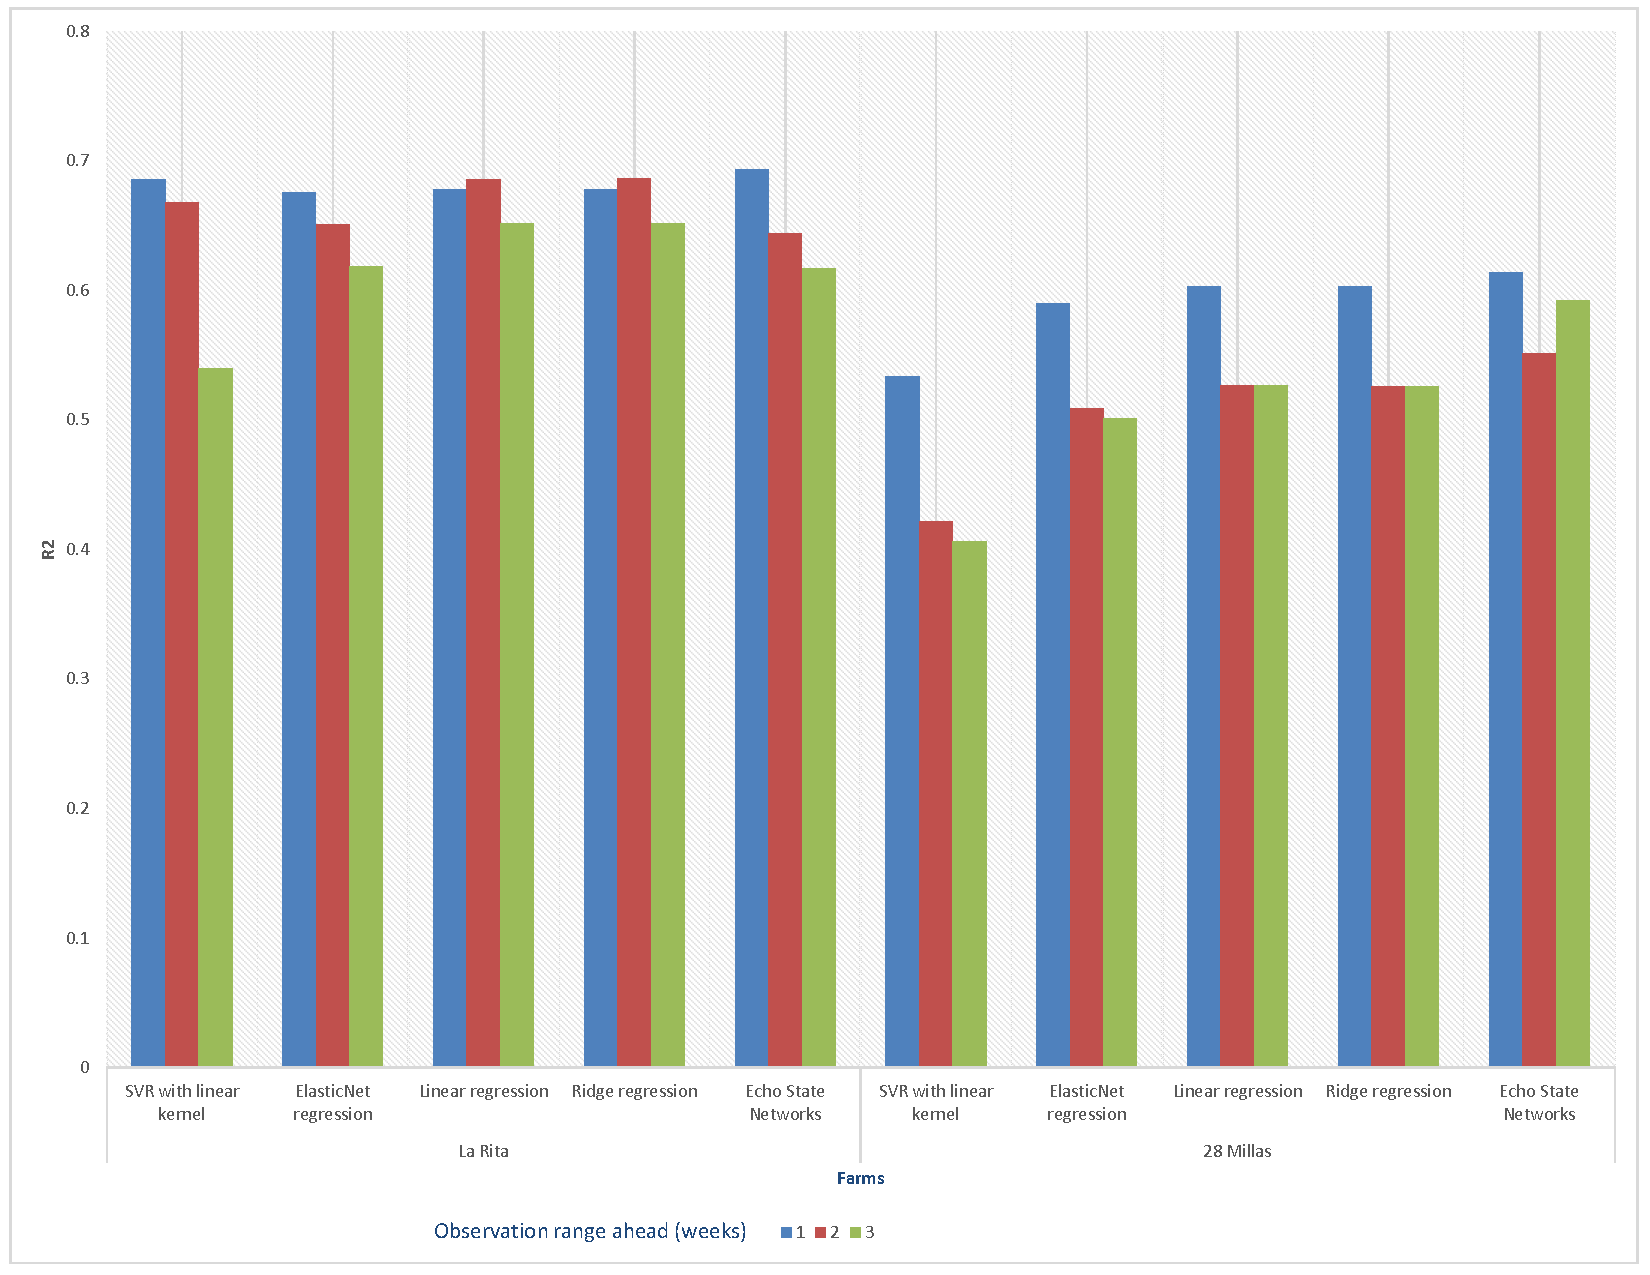
\includegraphics[scale=.5]{Phase_two_Best_R2_for_each_algortihm}
 \caption{Phase two - Best $R^2$ for each algorithm} 
 \label{figura8} 
\end{figure}

\figurename $.$\ref{figura9} presents, for one, two and three weeks ahead, the best $R^2$. Results are group by farm. The results confirms that, in general, to predict one week ahead is better than two weeks ahead, two than three and so on, this for both farms.

\begin{figure}[H] 
 \centering
 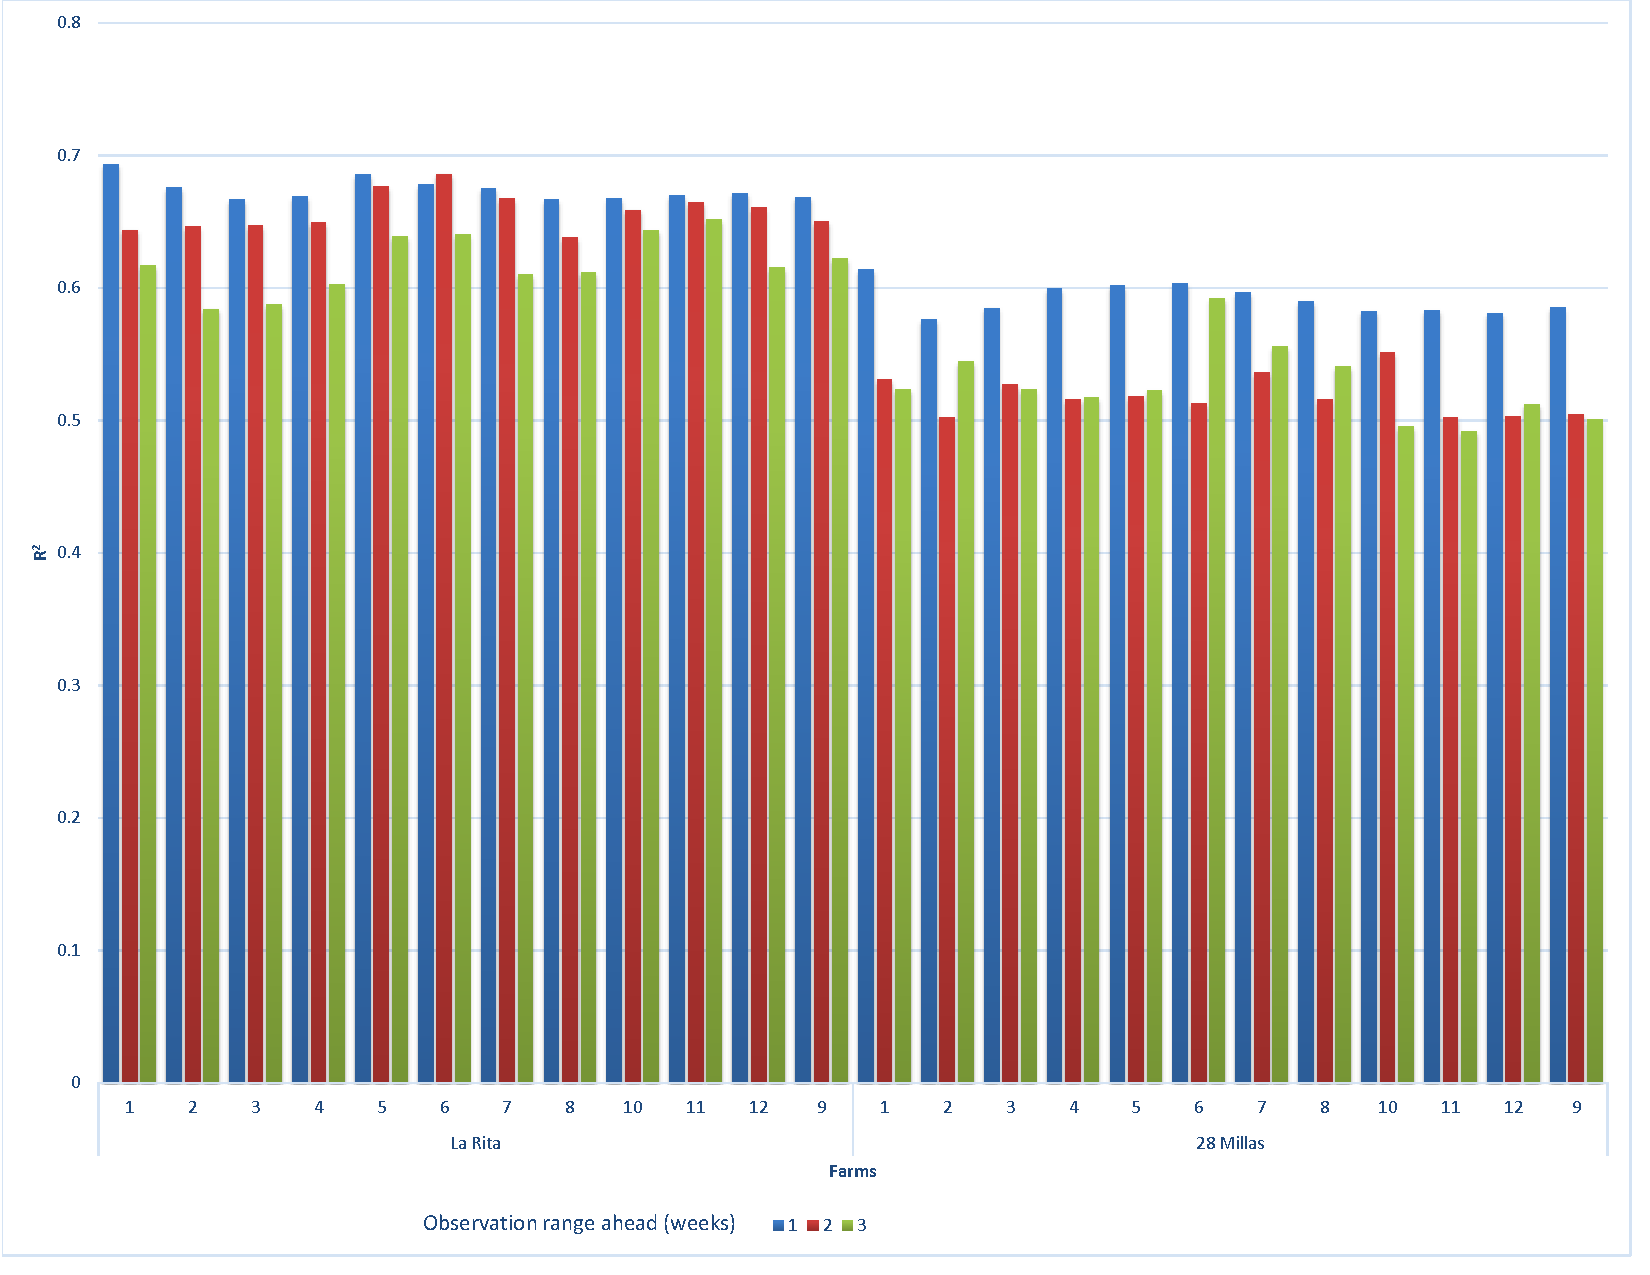
\includegraphics[scale=.5]{Phase_two_Best_R2_for_each_number_of_observation_range_in_the_patterm}
 \caption{Phase two - Best $R^2$ for each observation range} 
 \label{figura9} 
\end{figure}

\figurename $.$\ref{figura10} shows the best $R^2$ for each variables combination. Results are group by farm. This results confirm that $\overline{T}_{a}$ and the combination of $\overline{T}_{a}$ with $\overline{W}$, in both farms are the best variables combinations.

\begin{figure}[H] 
 \centering
 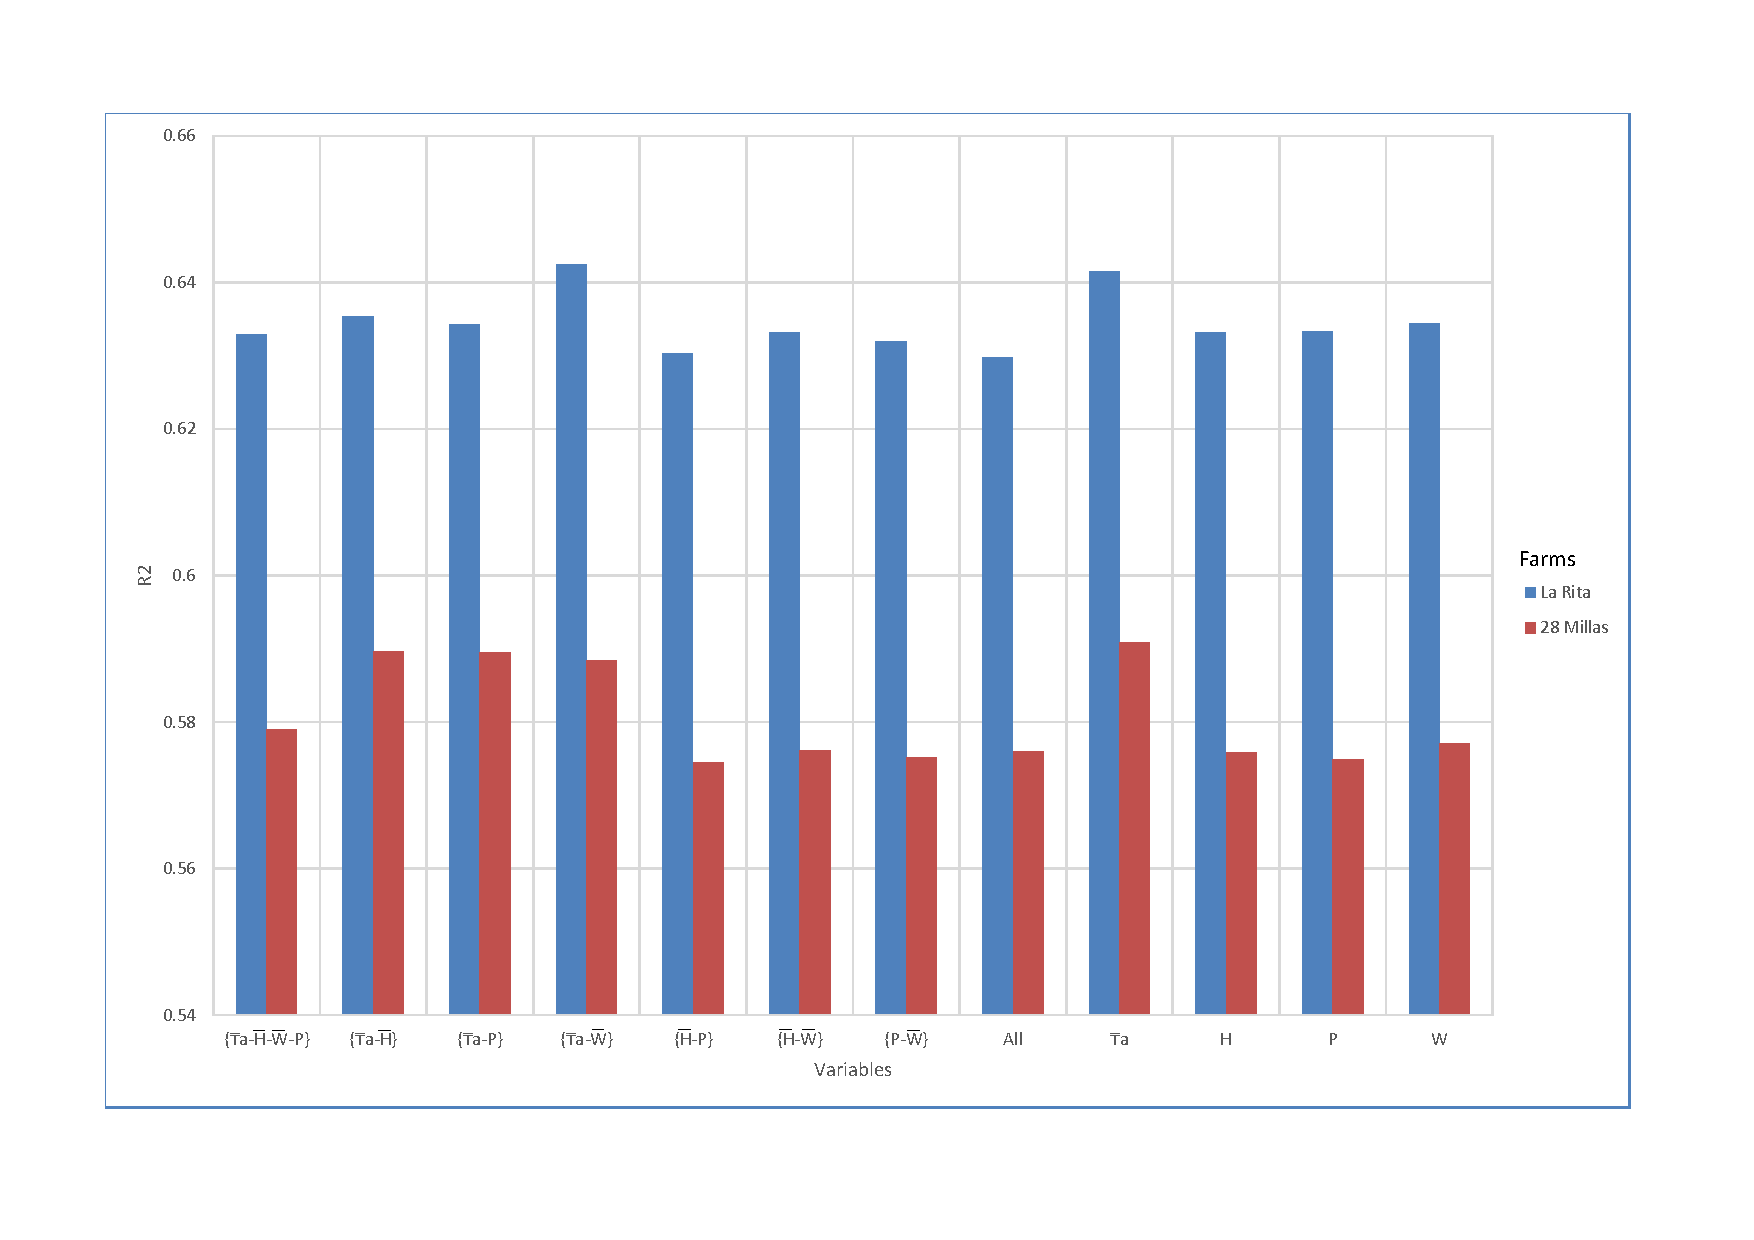
\includegraphics[scale=.5]{Phase_one_Best_R2_for_variables}
 \caption{Phase two - Best $R^2$ for each variable combination} 
 \label{figura10} 
\end{figure}

\figurename $.$\ref{figura11} shows the Pareto frontier for each farm with respect to $R^2$ and $RMSE$.  You can note that the behaviour of $R^2$ and $RMSE$ is similar to the phase one.

\begin{figure}[H] 
 \centering
 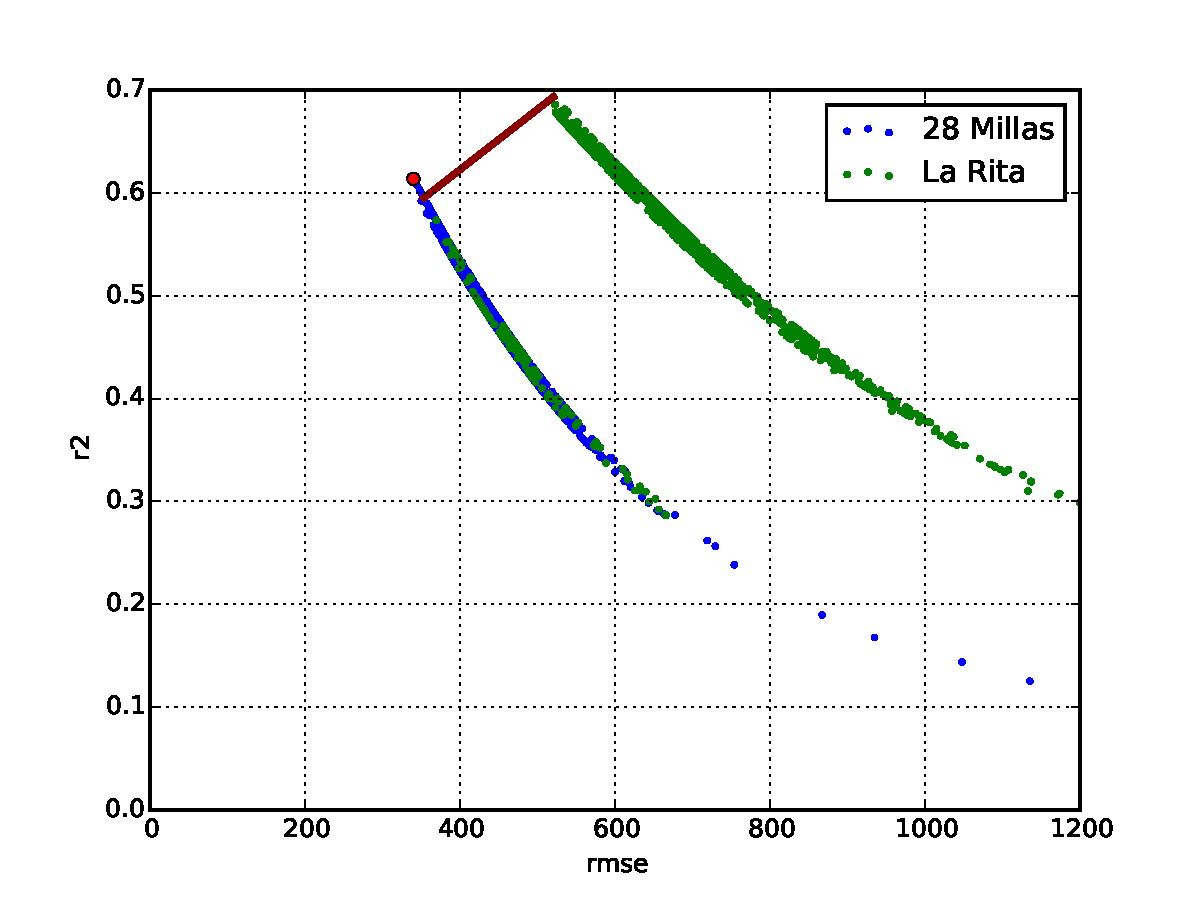
\includegraphics[scale=.8]{Phase_two_R2_RMSE}
 \caption{Phase two - Pareto frontier for $R^2$ and $RMSE$} 
 \label{figura11} 
\end{figure}


In phase two, the Pareto frontier for the La Rita farm is composed by 2 elements. The \tablename $.$\ref{tabla4} shows the composition about variables and observation ranges.

\begin{table}[h] 
\caption{Composition of the Pareto frontier - La Rita - Phase two} 
\label{tabla4} 
\centering
\begin{tabular}{c|c|c|c|c} 
\hline
\bfseries Variable & \bfseries Observation range & \bfseries Quantity & \bfseries Max $R^2$ & \bfseries Min $RMSE$\\ 
\hline\hline 
All & 1 to 1  & 2 & 69.33\% & 353.33 \\
\hline
\end{tabular} 
\end{table}

In 28 Millas Farm, the Pareto frontier is composed by 1 element. The \tablename $.$\ref{tabla5} details the result.

\begin{table}[h] 
\caption{Pareto frontier - 28 Millas - Phase two} 
\label{tabla5} 
\centering
\begin{tabular}{c|c|c|c|c} 
\hline
\bfseries Variable & \bfseries Observation range & \bfseries Quantity & \bfseries Max $R^2$ & \bfseries Min $RMSE$\\ 
\hline\hline 
Pair $\overline{T}_{a}$ $P$ & 1 to 1 & 1 & 61.36\% & 339.89 \\
\hline
\end{tabular} 
\end{table}

Again, similar to phase one, we can conclude that the best configuration in both farms is to consider the climate and the evolution stage of the current week to predict the evolution stage of the next week, one week to predict one week ahead with combinations of variables listed above.

\section{Acknowledgements}

The authors would like to thank Corbana S.A. for providing the data for this research. 

\section{References}

\bibliography{references}

\end{document}